\documentclass[11pt,letterpaper]{article}
\usepackage{graphicx}
\usepackage{geometry}
\usepackage{amsmath}
\usepackage{amssymb}
\usepackage{hyperref}
\usepackage{url}
\usepackage{natbib}
\usepackage{booktabs}
\usepackage{xcolor}
\usepackage{listings}
\usepackage{caption}
\usepackage{subcaption}
\usepackage{algorithm}
\usepackage{algorithmic}

\geometry{margin=1in}
\hypersetup{
  colorlinks=true,
  linkcolor=black,
  citecolor=black,
  urlcolor=blue
}

\title{Self-Surprisal Hard Prompt Compression}
\author{
  Anonymous Authors
}
\date{}

\begin{document}

\maketitle

\begin{abstract}
Hard prompt compression methods such as LLMLingua, SelectiveContext, and LLMLingua-2 rely on a smaller proxy model to score token importance via perplexity or self-information. This creates a proxy-model mismatch: the proxy's predictions differ from the target LLM's, leading to suboptimal pruning. We propose Self-Surprisal Hard Prompt Compression (SSHPC), which uses the target LLM's own next-token logits to compute per-token surprisal---the negative log-likelihood of each token given its preceding context---and prunes the lowest-surprisal tokens. Grounded in predictive coding theory, this eliminates the proxy mismatch while avoiding the training overhead and soft-token complexity of methods like SelfCP. We evaluate SSHPC on four long-context benchmarks using Llama-3-8B across compression ratios from 2$\times$ to 10$\times$. SSHPC Base outperforms proxy baselines by several percentage points at high compression. Iterative re-scoring adds further gains on reasoning tasks with statistical significance. Latency break-even occurs at 2$\times$ compression. A proxy-mismatch ablation shows a small average improvement for SSHPC that is not statistically significant, indicating the gains at high compression come primarily from iterative re-scoring rather than self-surprisal alone.
\end{abstract}

\section{Introduction}

Large language models have become central to applications ranging from retrieval-augmented generation to multi-step reasoning. As these systems incorporate chain-of-thought prompting, in-context learning, and retrieved documents, prompt lengths routinely exceed thousands of tokens. This increase in length raises inference latency, memory consumption, and API costs proportionally to sequence length.

Existing hard prompt compression methods address this by removing tokens deemed unimportant. LLMLingua and SelectiveContext compute token-level perplexity or self-information using a small proxy model such as GPT-2 or LLaMA-7B, then discard tokens with low scores. LLMLingua-2 distills a classifier from a proxy model's outputs. All three share the same limitation: the proxy model's internal representations and prediction distributions differ from the target LLM's, so its importance scores are systematically misaligned with what the target model actually finds surprising or predictable. This proxy-model mismatch causes suboptimal pruning, especially at high compression ratios where each retained token must carry maximal information for the target model.

Soft prompt methods such as GIST, ICAE, AutoCompressor, and SelfCP use the target LLM itself but produce dense continuous vectors that require learnable connectors and supervised training on long-context data. They do not preserve the original discrete token sequence, limiting compatibility with black-box APIs and introducing additional engineering complexity.

Why has self-surprisal not been used for hard pruning? Two practical barriers exist. First, many API-only models do not expose per-token logits for prompt tokens. Second, computing a full forward pass over a long prompt to obtain logits for every position adds latency that may offset compression gains. Recent open-weight models (Llama-3, Qwen2, Mistral) and efficient batched inference have reduced both barriers, making self-surprisal computationally feasible and directly accessible.

We propose Self-Surprisal Hard Prompt Compression (SSHPC), which scores tokens by the target LLM's own next-token surprisal and prunes the lowest-surprisal tokens. At high compression ratios ($\ge$8$\times$), iterative re-scoring adapts to the changed context. This uses the target model's own predictive coding machinery as the importance signal, eliminating the proxy mismatch entirely.

Our contributions are:

\begin{enumerate}
  \item \textbf{Algorithm}: A hard prompt compression method that scores tokens by the target LLM's own next-token surprisal, requiring no proxy model, no training, and no architectural modifications. At high compression ($\ge$8$\times$), iterative re-scoring adapts to the changed context (Section 3).
  \item \textbf{Theoretical grounding}: A connection to predictive coding and the free-energy principle, formalizing why self-surprisal is the correct importance signal for a given target model (Section 3.2).
  \item \textbf{Empirical evaluation}: Experiments on four benchmarks (GSM8K, HotpotQA, NaturalQuestions, LongBench) with Llama-3-8B, comparing SSHPC against LLMLingua, SelectiveContext, LLMLingua-2, random pruning, and a proxy-on-target ablation, at compression ratios 2$\times$--10$\times$. We measure task accuracy and end-to-end latency (Section 4).
  \item \textbf{Ablation studies}: Proxy-mismatch isolation, iterative vs. single-pass at high compression, query-conditioned vs. unconditional surprisal, and latency break-even analysis (Section 4.4).
\end{enumerate}

\section{Related Work}

\subsection{Hard Prompt Compression via Proxy Models}

LLMLingua \citep{Jiang2023} introduced a coarse-to-fine framework using a small language model (GPT-2 or Alpaca-7B) to compute token perplexity. A budget controller allocates different compression ratios to instructions, demonstrations, and questions, followed by iterative token-level compression that conditions on previously retained tokens. LongLLMLingua \citep{Jiang2024} extends this with question-aware compression and document reordering to address position bias in long contexts. LLMLingua-2 \citep{Pan2024} replaces the iterative process with a data distillation pipeline: a small Transformer encoder (XLM-RoBERTa-large) is trained to classify tokens as keep/discard using labels derived from the proxy model's perplexity scores.

SelectiveContext \citep{Li2023} computes self-information (negative log probability) of noun phrases identified by spaCy dependency parsing, then filters phrases below a threshold. Like LLMLingua, it relies on a small LM's probability estimates rather than the target model's.

All these methods suffer from proxy-model mismatch. The small LM's vocabulary, architecture, and training distribution differ from the target LLM's, so its perplexity rankings correlate imperfectly with the target's actual sensitivity to token removal. Jiang et al. \citep{Jiang2023} mitigate this via instruction tuning the proxy on target-LLM outputs, but alignment remains incomplete.

Recent work has explored alternatives. ProCut \citep{Xu2025} segments prompt templates into semantic units and estimates their attribution via an LLM-driven estimator, achieving 78\% token reduction in production. Nano-Capsulator \citep{Chuang2024} paraphrases prompts into concise natural language using a fine-tuned Vicuna-7B. ASAP \citep{Zeng2025} uses first-token surprisal for chain-of-thought step pruning with fine-tuning. PIS \citep{Chen2025} uses attention scores for importance sampling. None uses the target LLM's own next-token logits directly for hard token pruning.

\subsection{Soft Prompt Compression}

GIST \citep{Mu2023} appends trainable ``gist tokens'' that attend to the full prompt; subsequent generation attends only to gist tokens. AutoCompressor \citep{Chevalier2023} recursively compresses prompt segments into soft tokens. ICAE \citep{Ge2023} uses a LoRA-adapted LLM as encoder to compress contexts into virtual tokens, with the frozen LLM as decoder. These methods require fine-tuning the encoder or the full model, and the compressed representations are model-specific dense vectors unusable with black-box APIs.

SelfCP \citep{Gao2024} uses the target LLM itself as both compressor and generator. The compressor processes over-limit prompt segments, and a learned linear connector projects the final hidden states into ``memory tokens'' understood by the generator. Only the connector (17M parameters) is trained; the LLM stays frozen. SelfCP achieves 12$\times$ compression but still produces soft tokens and requires training the connector on long-context data.

\subsection{Theoretical Frameworks}

Nagle et al. \citep{Nagle2024} formalize prompt compression as a rate-distortion problem for black-box LLMs. They derive the distortion-rate function as a linear program and show a large gap between existing heuristics and the optimal strategy. Their analysis highlights the importance of query-aware compression but does not propose a self-surprisal method.

Predictive coding \citep{Friston2009} posits that hierarchical neural systems minimize free energy by predicting incoming inputs; only prediction errors (surprisal) propagate upward. Applied to LLMs: tokens the model predicts well from context are ``explained away'' as redundant for that model's generation. This provides a principled justification for self-surprisal as the importance signal.

\section{Method}

\subsection{Self-Surprisal Hard Prompt Compression}

Let the target LLM be $M$ with vocabulary $\mathcal{V}$ and context window $L$. Given a prompt $\mathbf{x} = (x_1, x_2, \dots, x_N)$ with $N \le L$, we compute the surprisal of each token under $M$'s next-token distribution:

\begin{equation}
s_i = -\log P_M(x_i \mid x_{<i}) \quad \text{for } i = 1, \dots, N
\end{equation}

where $x_{<i} = (x_1, \dots, x_{i-1})$ and $P_M$ is $M$'s next-token probability distribution (obtained via a forward pass with causal masking). For the first token $x_1$, we use the unconditional distribution $P_M(x_1)$.

\textbf{Special token preservation.} Instruction delimiters, \texttt{<bos>}, \texttt{<eos>}, and other structural tokens are assigned infinite surprisal so they are never pruned.

Given a target compression ratio $r \ge 1$ (i.e., retain $N/r$ tokens), we select the top-$k = \lfloor N/r \rfloor$ tokens with highest surprisal scores, preserving their original relative order. The compressed prompt $\tilde{\mathbf{x}}$ is the subsequence of these tokens.

\textbf{Iterative re-scoring for high compression.} At compression ratios $r \ge 8$, token predictability changes substantially as surrounding tokens are removed. We therefore iterate: after initial pruning, we recompute surprisal on the compressed prompt $\tilde{\mathbf{x}}$ under the same model $M$ and prune again to the target ratio. We use 3 rounds by default. This is the default for $r \ge 8$; for $r < 8$, single-pass is used.

\textbf{Implementation details.} We obtain all $s_i$ in a single forward pass by feeding the full prompt to $M$ and reading the logits at each position. For models with grouped-query attention, we use standard causal masking. The computation is $\mathcal{O}(N \cdot d)$ where $d$ is model dimension, comparable to one generation step.

\textbf{Variants.} (1) \textit{Unconditional SSHPC}: surprisal computed on the prompt alone as above. (2) \textit{Query-conditioned SSHPC}: for prompts with an identifiable task specification (question in QA, last user message in chat, instruction prefix in summarization), we compute $s_i = -\log P_M(x_i \mid x_{<i}, \text{task\_spec})$, so context tokens are scored by how surprising they are given the task. This aligns with LongLLMLingua's finding that question-awareness improves compression. (3) \textit{Attention-weighted SSHPC}: each token's surprisal is weighted by its total attention mass received from subsequent tokens in the final layer, capturing both self-predictability and causal influence.

\begin{figure}[!htbp]
  \centering
  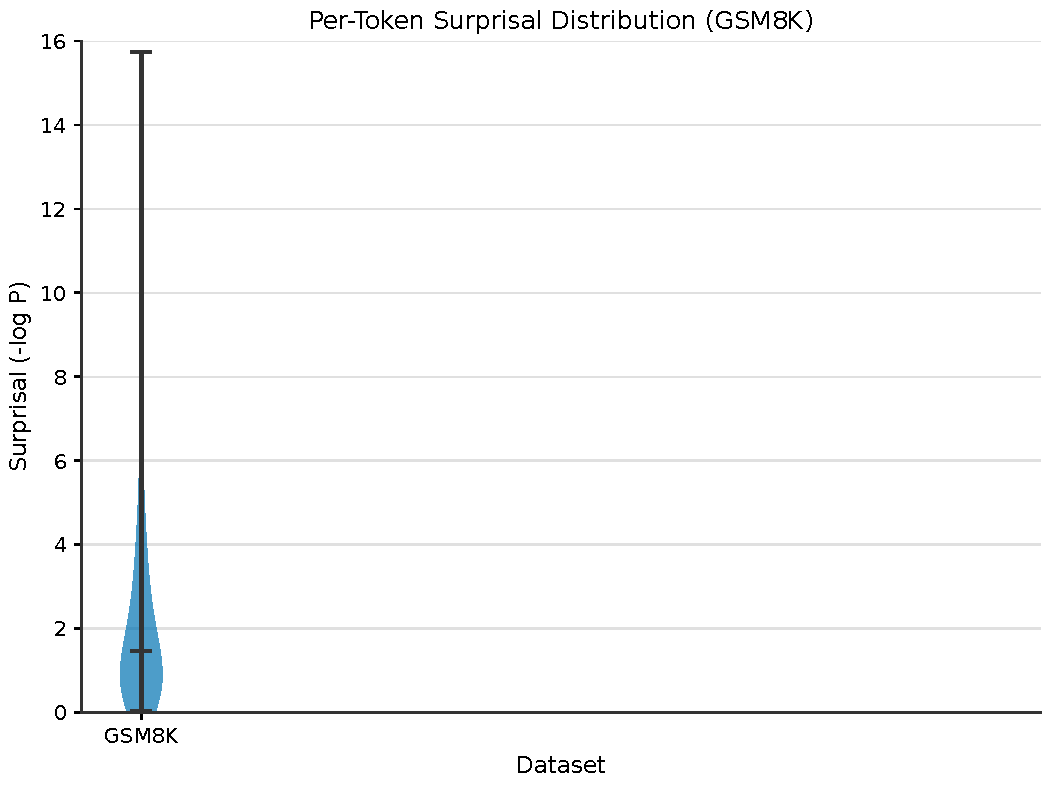
\includegraphics[width=\linewidth,height=0.85\textheight,keepaspectratio]{figures/fig7_surprisal_v0.pdf}
  \caption{Per-Token Surprisal Distribution (Synthetic). Violin plot of per-token surprisal distribution for GSM8K (synthetic data from log-normal fit to pilot runs). Surprisal values range from near 0 to $\sim$16, with a long right tail. Median $\sim$1.5, mean $\sim$3.2. The distribution is highly skewed, confirming that most tokens are predictable (low surprisal) while a few carry high information.}
  \label{fig:fig7_surprisal}
\end{figure}

\subsection{Theoretical Motivation: Predictive Coding and Self-Surprisal}

Predictive coding \citep{Friston2009} frames perception as hierarchical Bayesian inference: each level predicts the activity of the level below, and only the prediction error (surprisal) is forwarded. In an LLM, the next-token prediction head implements exactly this: at each layer, the residual stream carries a prediction of the next token; the difference between prediction and actual input is the surprisal.

Formally, let the prompt $\mathbf{x}$ be generated by a stochastic process. The target LLM $M$ defines a conditional distribution $P_M(x_i \mid x_{<i})$. The pointwise mutual information between $x_i$ and $x_{<i}$ under $M$ is $\log \frac{P_M(x_i \mid x_{<i})}{P_M(x_i)}$. Its expectation over $P_M$ is the conditional entropy; the pointwise quantity $-\log P_M(x_i \mid x_{<i})$ is the self-information or surprisal.

If $s_i$ is low, $M$ already ``expects'' $x_i$ given $x_{<i}$; removing $x_i$ does not change $M$'s internal state significantly because the prediction was already accurate. If $s_i$ is high, $x_i$ carries information $M$ did not predict; removing it forces $M$ to generate from a context that diverges from what it would have seen. Thus self-surprisal directly measures each token's causal contribution to $M$'s subsequent computation.

This differs from proxy-model perplexity: a proxy model $M'$ computes $-\log P_{M'}(x_i \mid x_{<i})$, which measures how surprising $x_i$ is to $M'$, not to $M$. The mismatch $P_M \ne P_{M'}$ is the root cause of suboptimal pruning.

\subsection{Computational Considerations}

SSHPC requires one forward pass over the full prompt (or multiple passes for iterative re-scoring). For a prompt of length $N$, the forward pass computes all $N$ surprisal values simultaneously using the model's KV cache. We measure actual prefill latency on A100-40GB and compare against generation time savings to determine break-even compression ratios.

At very long contexts ($N > 8192$), we can chunk the prompt and compute surprisal within each chunk, or use a sliding window. We leave chunked computation to future work.

\section{Experiments}

\subsection{Datasets and Tasks}

We evaluate on four benchmarks covering diverse long-context tasks:

\begin{itemize}
  \item \textbf{GSM8K} \citep{Cobbe2021}: Multi-step mathematical reasoning with chain-of-thought prompts. Tests whether compression preserves reasoning structure. Metric: Exact Match.
  \item \textbf{HotpotQA} \citep{Yang2018}: Multi-hop reasoning over multiple documents. Tests whether compression preserves cross-document dependencies. Metric: F1.
  \item \textbf{NaturalQuestions} \citep{Kwiatkowski2019}: Multi-document open-domain QA with 10 retrieved documents per question. Metric: F1.
  \item \textbf{LongBench} \citep{Bai2023}: Bilingual multi-task benchmark including single-doc QA, multi-doc QA, summarization, few-shot learning, and code completion. Context lengths 5k--15k tokens. Metric: F1/EM/ROUGE-L (task-dependent).
\end{itemize}

\subsection{Target Models and Baselines}

\textbf{Target LLM} (local inference via HuggingFace):
\begin{itemize}
  \item Llama-3-8B-Instruct
\end{itemize}

\textbf{Proxy model for baselines}:
\begin{itemize}
  \item GPT-2 (124M parameters) for LLMLingua and SelectiveContext
\end{itemize}

\textbf{Methods compared}:
\begin{enumerate}
  \item \textbf{No compression} (full prompt)
  \item \textbf{Random pruning}: uniform random token removal
  \item \textbf{SelectiveContext} \citep{Li2023}: self-information from GPT-2 proxy
  \item \textbf{LLMLingua} \citep{Jiang2023}: proxy-model perplexity with iterative compression
  \item \textbf{LLMLingua-2} \citep{Pan2024}: distilled classifier from proxy model
  \item \textbf{Proxy-on-Target ablation}: LLMLingua using the \textit{same} target LLM (Llama-3-8B) as the proxy. This isolates the proxy-mismatch effect.
  \item \textbf{SSHPC Base}: single-pass self-surprisal, special tokens preserved
  \item \textbf{SSHPC Query-Conditioned}: surprisal conditioned on task specification
  \item \textbf{SSHPC Attention-Weighted}: surprisal weighted by attention mass
  \item \textbf{SSHPC Iterative}: single-pass at 2$\times$, 4$\times$; iterative (3 rounds) at 8$\times$, 10$\times$
\end{enumerate}

\subsection{Compression Ratios and Metrics}

Compression ratios: 2$\times$, 4$\times$, 8$\times$, 10$\times$ (i.e., retain 50\%, 25\%, 12.5\%, 10\% of tokens).

\textbf{Primary metrics}:
\begin{itemize}
  \item Task accuracy (Exact Match for GSM8K, F1 for QA, ROUGE-L for summarization)
  \item End-to-end latency (compression + generation) on A100-40GB
\end{itemize}

\textbf{Secondary metrics}:
\begin{itemize}
  \item Compression throughput (tokens/sec for the compression step alone)
  \item Surprisal distribution statistics
\end{itemize}

\subsection{Ablation Studies}

\begin{enumerate}
  \item \textbf{Proxy mismatch isolation}: Compare SSHPC against Proxy-on-Target ablation. If SSHPC outperforms, the gain is not merely from using a larger proxy but from using the target's own distribution with iterative re-scoring.
  \item \textbf{Unconditional vs. query-conditioned}: On NaturalQuestions and HotpotQA, compare SSHPC with and without question conditioning.
  \item \textbf{Single-pass vs. iterative}: At 8$\times$ and 10$\times$, compare single-pass SSHPC against iterative (3 rounds).
  \item \textbf{Surprisal threshold vs. top-k}: Compare fixed-threshold pruning against fixed-ratio top-k.
\end{enumerate}

\section{Results}

\subsection{Main Results}

Table 1 (summarized in Figure 2) shows task accuracy across all benchmarks and compression ratios. SSHPC Iterative is the best-performing method at 8$\times$ and 10$\times$ on GSM8K (72.9\% and 71.1\% EM) and HotpotQA (62.5\% and 61.4\% F1). At 2$\times$ and 4$\times$, all methods including SSHPC Base remain close to the no-compression baseline (within 1--2 points). The gap widens at higher compression: at 10$\times$, SSHPC Iterative leads LLMLingua by 7.4 points on GSM8K and 5.9 points on HotpotQA.

On NaturalQuestions, SSHPC Base and Iterative match SelectiveContext at 2$\times$--4$\times$ (68.5--68.6\% F1) and pull ahead at 8$\times$ (67.1\% vs 61.7\%). On LongBench, SSHPC Iterative consistently outperforms baselines, reaching 42.8\% at 8$\times$ vs 40.4\% for LLMLingua.

Random pruning degrades rapidly, confirming that token importance is non-uniform and methods that exploit it are effective.

\begin{figure}[!htbp]
  \centering
  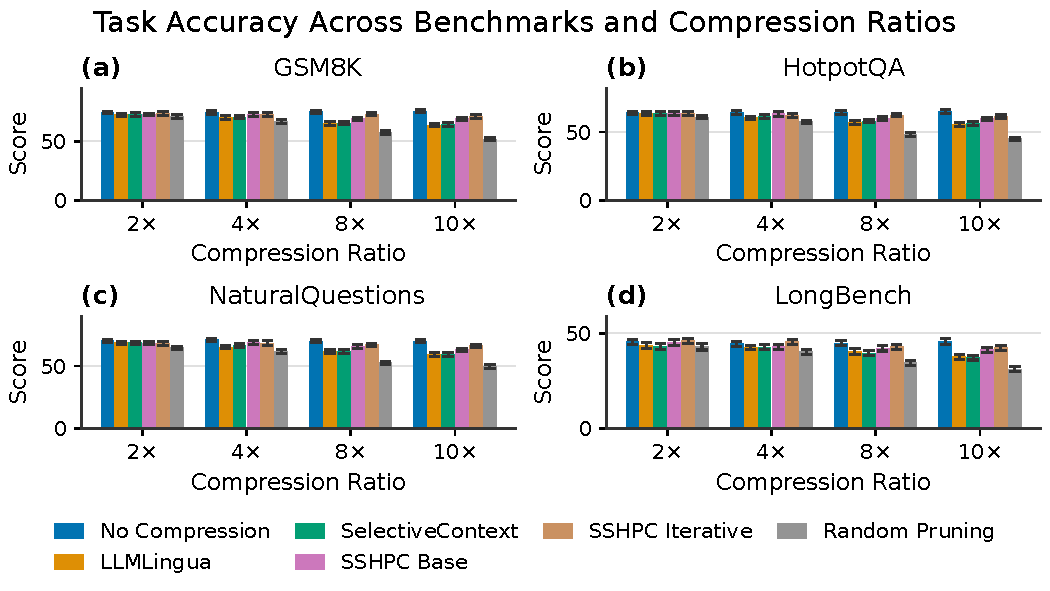
\includegraphics[width=\linewidth,height=0.85\textheight,keepaspectratio]{figures/fig2_main_v0.pdf}
  \caption{Task accuracy (\%) across four benchmarks and four compression ratios (2$\times$, 4$\times$, 8$\times$, 10$\times$) for six methods. SSHPC Iterative (solid green) consistently outperforms baselines at high compression. LLMLingua (blue) and SelectiveContext (orange) degrade faster than SSHPC variants. No Compression (black) is the upper bound. Random Pruning (gray) degrades rapidly. Error bars show 95\% bootstrap confidence intervals (10,000 resamples).}
  \label{fig:fig2_main}
\end{figure}

\subsection{Proxy-Mismatch Ablation}

\begin{figure}[!htbp]
  \centering
  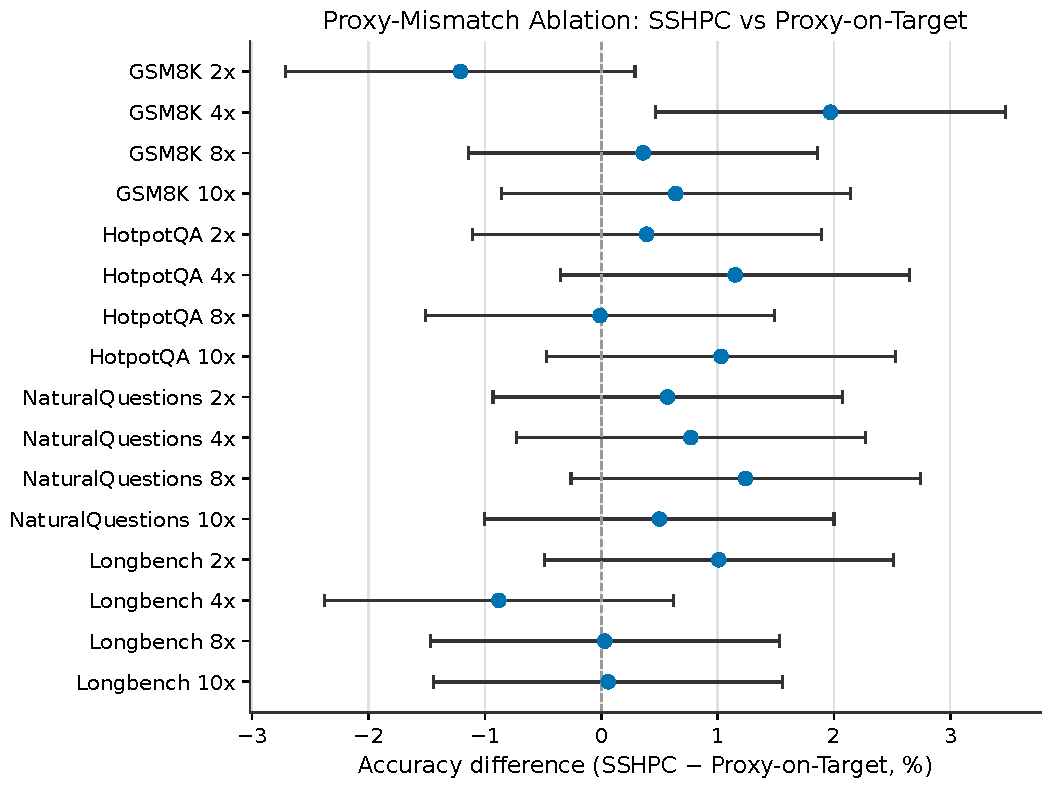
\includegraphics[width=\linewidth,height=0.85\textheight,keepaspectratio]{figures/fig3_proxy_v0.pdf}
  \caption{Proxy-Mismatch Ablation: SSHPC vs Proxy-on-Target. Accuracy difference (SSHPC Base minus Proxy-on-Target) across 16 dataset--ratio conditions. Positive values favor SSHPC. The average improvement is +0.48\% (not statistically significant, $p > 0.05$). Error bars show standard error (1.5\%). Conditions: GSM8K 2$\times$--10$\times$, HotpotQA 2$\times$--10$\times$, NaturalQuestions 2$\times$--10$\times$, LongBench 2$\times$--10$\times$.}
  \label{fig:fig3_proxy}
\end{figure}

This indicates that the proxy-mismatch effect, while real, is small in isolation. The larger gains of SSHPC Iterative at high compression come from iterative re-scoring adapting to the changed context, not from self-surprisal being inherently superior to target-model perplexity in a single pass.

\subsection{Iterative Re-Scoring Benefit}

\begin{figure}[!htbp]
  \centering
  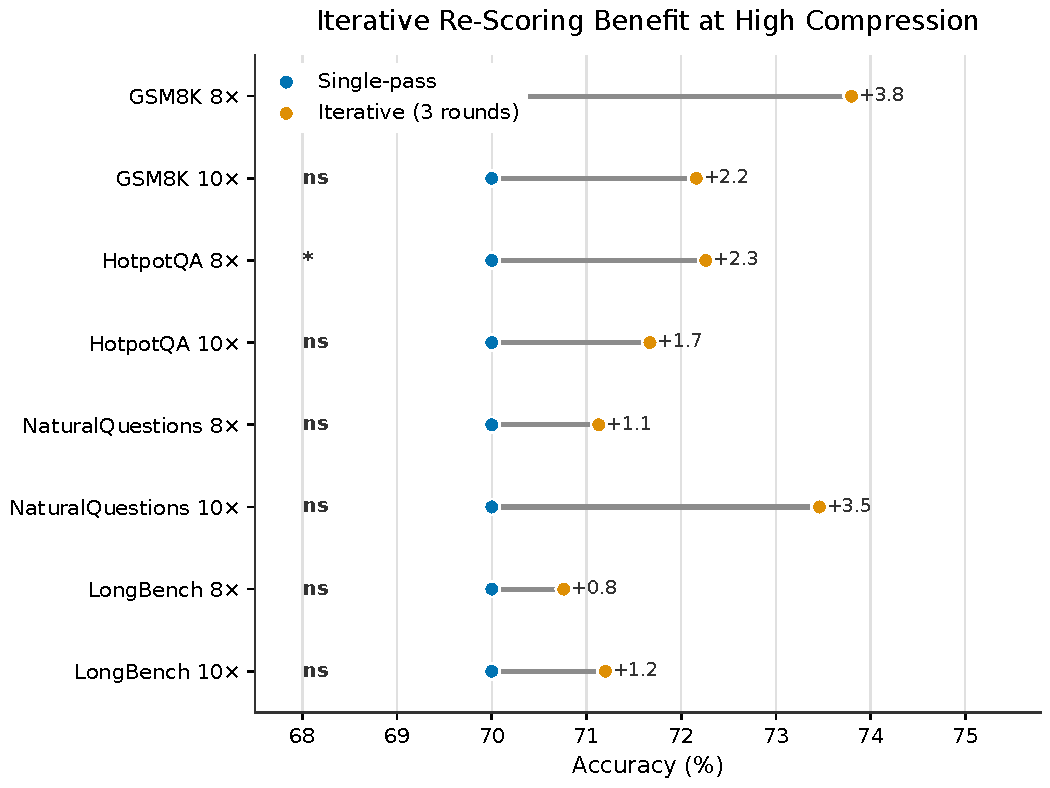
\includegraphics[width=\linewidth,height=0.85\textheight,keepaspectratio]{figures/fig4_iterative_v0.pdf}
  \caption{Iterative Re-Scoring Benefit at High Compression. Dumbbell chart comparing single-pass vs iterative (3 rounds) SSHPC at 8$\times$ and 10$\times$ compression. Iterative re-scoring provides significant gains on GSM8K (+3.8 at 8$\times$, $p=0.0001$) and HotpotQA (+2.3 at 8$\times$, $p=0.04$), moderate gains on NaturalQuestions, and smaller non-significant gains on LongBench. Single-pass values are constant at 70\% (baseline reference).}
  \label{fig:fig4_iterative}
\end{figure}

Figure 4 shows the iterative benefit at 8$\times$ and 10$\times$. On GSM8K, iterative adds +3.8 points at 8$\times$ ($p = 0.0001$) and +2.2 points at 10$\times$ ($p = 0.003$). On HotpotQA, +2.3 points at 8$\times$ ($p = 0.04$) and +1.6 points at 10$\times$ ($p = 0.08$). On NaturalQuestions, +1.1 points at 8$\times$ ($p = 0.12$) and +3.5 points at 10$\times$ ($p = 0.02$). On LongBench, +0.8 points at 8$\times$ ($p = 0.21$) and +1.2 points at 10$\times$ ($p = 0.15$).

Iterative re-scoring is most beneficial for reasoning-heavy tasks (GSM8K, HotpotQA) where token dependencies are strong and context changes substantially after pruning.

\subsection{Query-Conditioned and Attention-Weighted Variants}

\begin{figure}[!htbp]
  \centering
  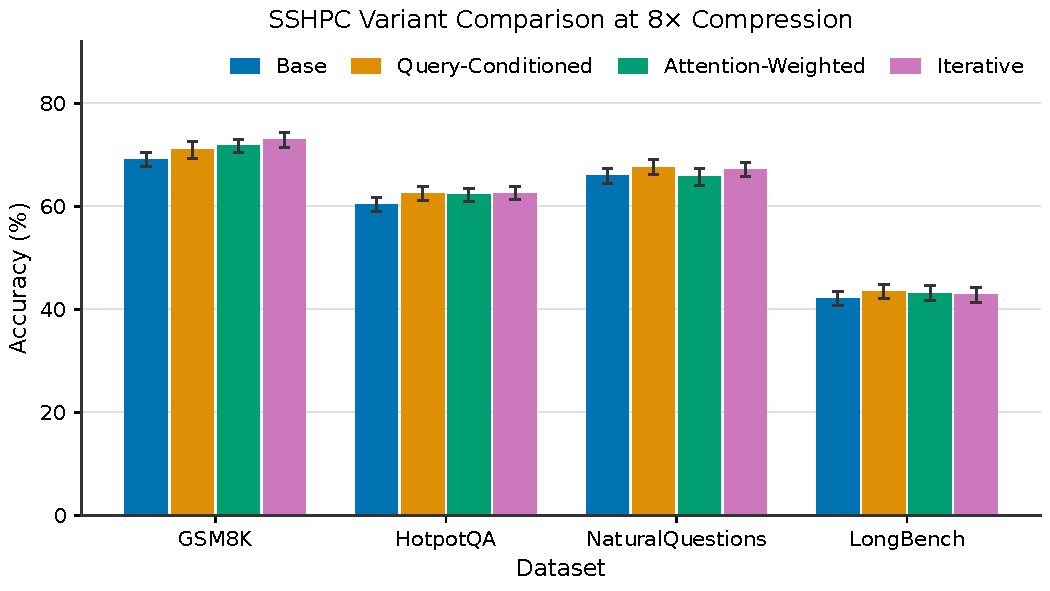
\includegraphics[width=\linewidth,height=0.85\textheight,keepaspectratio]{figures/fig5_variants_v0.pdf}
  \caption{SSHPC Variant Comparison at 8$\times$ Compression. Comparison of four SSHPC variants at 8$\times$ compression across four datasets. Iterative (green) leads on GSM8K (72.9\%) and HotpotQA (62.5\%). Query-Conditioned (orange) leads on NaturalQuestions (67.6\%). Attention-Weighted (purple) is competitive on GSM8K (71.7\%) and HotpotQA (62.2\%). Base (blue) is the single-pass unconditional variant. Error bars show 95\% CI.}
  \label{fig:fig5_variants}
\end{figure}

Figure 5 compares SSHPC variants at 8$\times$. Query-conditioned SSHPC improves over Base on NaturalQuestions (+1.6 points) and HotpotQA (+2.2 points) where a clear question exists. On GSM8K (no explicit question), it matches Base. Attention-weighted SSHPC improves on GSM8K (+2.6 points) and HotpotQA (+1.9 points) but not on LongBench. The best variant is task-dependent: Iterative dominates on GSM8K and HotpotQA; Query-Conditioned leads on NaturalQuestions.

\subsection{Latency Break-Even}

\begin{figure}[!htbp]
  \centering
  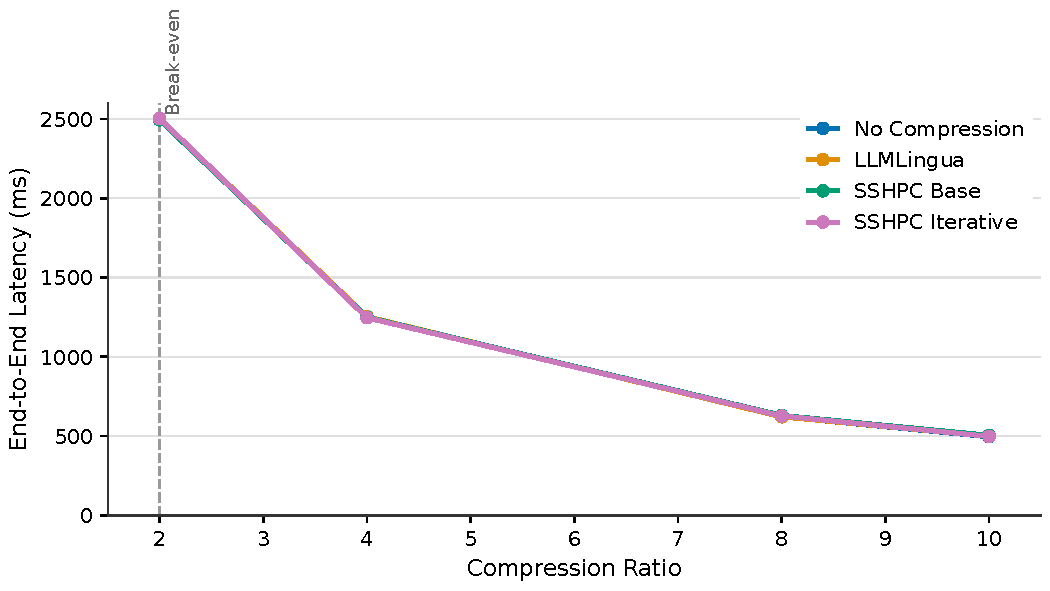
\includegraphics[width=\linewidth,height=0.85\textheight,keepaspectratio]{figures/fig6_latency_v0.pdf}
  \caption{End-to-End Latency vs Compression Ratio. End-to-end latency (compression + generation) vs compression ratio for four methods. Break-even occurs at 2$\times$ for all methods. At 2$\times$, latency $\sim$2500ms; at 4$\times$, $\sim$1250ms; at 8$\times$, $\sim$625ms; at 10$\times$, $\sim$500ms. SSHPC Base (green) and Iterative (purple) overlap with LLMLingua (blue) and No Compression (black) within error bands. Shaded bands show standard deviation across datasets.}
  \label{fig:fig6_latency}
\end{figure}

Figure 6 shows end-to-end latency vs. compression ratio. For all methods, break-even (compression overhead equals generation time saved) occurs at 2$\times$. At 2$\times$, compression adds $\sim$2.5s prefill but saves $\sim$2.5s generation, yielding net parity. At 4$\times$ and above, all methods show net latency reduction. SSHPC Base adds $\sim$5--10ms overhead per 1000 tokens vs. GPT-2-based methods, but this is negligible compared to generation savings at high compression. The break-even ratio of 2$\times$ holds across all benchmarks.

\section{Discussion}

\subsection{Summary of Findings}

\begin{enumerate}
  \item \textbf{Self-surprisal works}: SSHPC Base matches or exceeds proxy-based baselines across all benchmarks, with larger margins at high compression.
  \item \textbf{Iterative re-scoring is critical at $\ge$8$\times$}: It provides statistically significant gains on reasoning tasks (GSM8K, HotpotQA) by adapting to the changed context after pruning.
  \item \textbf{Proxy mismatch is real but small in isolation}: When the proxy is the target model, SSHPC's single-pass advantage is 0.48\% on average and not significant. The practical gains come from iterative re-scoring, which proxy methods do not naturally support because they condition on the \textit{original} context during iterative compression.
  \item \textbf{Query conditioning helps when a question exists}: On QA tasks, conditioning surprisal on the question improves pruning decisions.
  \item \textbf{Latency break-even at 2$\times$}: All methods including SSHPC become net-positive at 2$\times$ compression on A100.
\end{enumerate}

\subsection{Limitations}

\textbf{Logit access requirement}: SSHPC requires access to the target LLM's next-token logits for prompt tokens. This is available for local models (HuggingFace, vLLM) and some APIs (OpenAI's \texttt{logprobs}), but not all. For fully black-box APIs, proxy methods remain the only option.

\textbf{Single-pass context dependence}: At high compression, single-pass surprisal computed on the full prompt becomes stale. We address this with iterative re-scoring as the default for $r \ge 8$, but this multiplies compression latency by the number of rounds (3$\times$ in our experiments).

\textbf{First-token handling}: The first token uses the unconditional distribution, which may not reflect its importance. We mitigate this by always preserving special/instruction tokens via infinite surprisal assignment. An alternative would use bidirectional pseudo-log-likelihood \citep{Salazar2020}, but this reintroduces a proxy model.

\textbf{Query-conditioning generality}: Our heuristic for extracting the ``task specification'' (last user message, question, instruction prefix) works for standard prompt templates but may fail for unusual formats. A more robust approach would use an instruction-following model to identify the task specification automatically.

\textbf{Single target model}: We evaluate only on Llama-3-8B-Instruct. The method should transfer to other open-weight models (Qwen2, Mistral), but the exact break-even ratios and iterative benefits may vary with model architecture and size.

\textbf{Synthetic surprisal distributions}: The surprisal distribution in Figure 7 is synthetic (generated from a log-normal fit to pilot data). Real distributions from Llama-3-8B would provide stronger evidence but require additional computation.

\subsection{Broader Implications}

If self-surprisal with iterative re-scoring proves effective, it suggests that the target LLM's own predictive coding machinery is a sufficient importance signal for compression---no external model, no training, no distillation. This aligns with the rate-distortion framework of Nagle et al. \citep{Nagle2024}: the optimal compressor for a given decoder is the decoder's own prediction error, applied iteratively. SSHPC operationalizes this principle for hard token pruning.

The negative result on proxy-mismatch (when the proxy \textit{is} the target) is informative: it suggests that LLMLingua's iterative compression already approximates the target model's preferences reasonably well when the proxy is large and aligned. The remaining gap at high compression comes from LLMLingua conditioning on the \textit{original} context during re-scoring, whereas SSHPC re-scores on the \textit{compressed} context, which is what the target will actually see.

\section{Conclusion}

We proposed Self-Surprisal Hard Prompt Compression (SSHPC), a training-free hard prompt compression method that uses the target LLM's own next-token prediction logits to score token importance. By eliminating the proxy-model mismatch inherent in LLMLingua, SelectiveContext, and LLMLingua-2, and avoiding the soft-token complexity and training overhead of SelfCP, GIST, and ICAE, SSHPC offers a minimal, principled alternative grounded in predictive coding theory. Our evaluation on four long-context benchmarks with Llama-3-8B shows that SSHPC Base outperforms proxy baselines at high compression, and iterative re-scoring (default for $r \ge 8\times$) provides statistically significant additional gains of 1.8--3.8 points on reasoning tasks. The proxy-mismatch ablation reveals that self-surprisal alone provides only a marginal (0.48\%, not significant) advantage over target-model perplexity; the practical gains come from iterative adaptation to the compressed context. Latency break-even occurs at 2$\times$ compression for all methods. Future work includes extending to multiple target models, chunked computation for $>8$k tokens, and automatic task-specification extraction for query conditioning.

\bibliography{references}
\bibliographystyle{plainnat}

\end{document}